
% Eigener Beitrag: Beschreibung, Begründung, Aufzeigung, Methode, Fazit

\chapter{Anforderungsanalyse}
\label{sec:anforderungsanalyse}
\todo{intro}

\section{Anforderungsanalyse des Programmes}
\todo{intro}

\subsection{Stakeholders}
\label{sec:anforderungsanalyse:stakeholders}
In der \cref{fig:anfoderungsanalyse:stakeholders} sind die Stakeholders des Projekt abgebildet.
\begin{table}[h] 
	\caption{Stakeholders}
	\centering
	\rowcolors{1}{tablebodycolor}{tablerowcolor}
	\label{fig:anfoderungsanalyse:stakeholders}
	\begin{tabular}{ | c | L{5cm} | L{5cm} | } 
		\hline 
		\rowcolor{tableheadcolor}
		\bfseries Stakeholder & \bfseries Beschreibung & \bfseries Erwartungen \\ \hline 
		%Kunde & Besucher der Webseite, welcher Objekte buchen möchte und Werbung wahrnimmt. & Durch das Projekt sollen ihm passendere Objekte und Vorschläge angezeigt werden. \\ \hline 
		Interhome Marketing & Das Marketing ist für die Werbung auf der Interhome Webseite verantwortlich. & Möchte auf der Webseite passendere Angebote dem Benutzer darstellen.  \\ \hline 
		Interhome Einkauf & Abteilung welche die Objekte einkauft welche auf der Interhome Webseite dargestellt werden. & Sie sollen durch das Projekt den Kunden besser verstehen und somit die Objekte einkaufen, welche von den Kunden gewünscht sind. \\ \hline 
		Interhome Tester & Testet das Programm und gibt Feedback ob es korrekt arbeitet. & Eine gut entwickeltes Programm welches bereits grundlegend von der Hotelplan Entwicklung getestet wurde. \\ \hline 
		Hotelplan Entwickler & Verantwortlich für die Umsetzung dieses Projektes. & Eine reibungslose Umsetzung des Projektes sowie eine konstruktive Kooperation mit den Testern. \\ \hline 
	\end{tabular}
\end{table} 

\subsection{Anwendungsfälle}
\label{sec:anforderungsanalyse:anwendungsfaelle}
In der \cref{fig:anfoderungsanalyse:anwendungsfaelle:1} werden die Anwendungsfälle des Programmes dargestellt. Die Aktoren sind von der \cref{fig:anfoderungsanalyse:stakeholders} übernommen worden. Nachfolgend werden die einzelnen Anwendungsfälle beschrieben.
\begin{figure}[H]
	\RawFloats
	\centering
	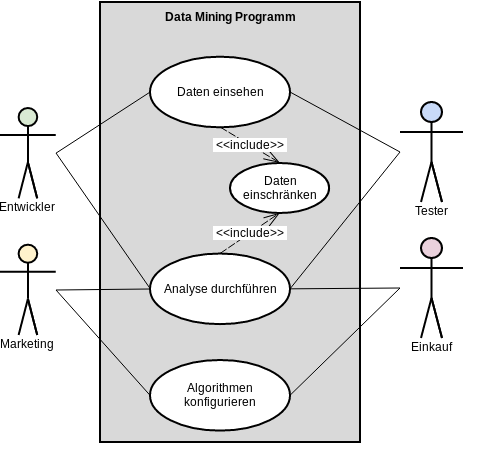
\includegraphics[width=0.7\textwidth]{images/usecase}
	\caption{Anwendungsfälle}
	\label{fig:anfoderungsanalyse:anwendungsfaelle:1}
\end{figure}

\paragraph{Daten einschränken} Es muss möglich sein, die Daten einzuschränken. Dies sollte über vordefinierte Filterkriterien geschehen die vom Benutzer ausgewählt werden können.

\paragraph{Daten einsehen} Um ein Überblick über die gesamten Daten zu haben und um einen Algorithmus zu überprüfen, soll eine Ansicht erstellt werden welche die Daten unbearbeitet darstellt. Sie sollen jedoch gefiltert werden können damit man die selbe Einschränkung vornehmen kann welche auch bei den Algorithmen eingestellt werden kann.

\paragraph{Analyse durchführen} Es sollte möglich sein, einen oder mehrere Algorithmen auf die Daten anzuwenden und so eine Analyse durchzuführen. Die Daten sollen initial eingeschränkt werden können um nur eine Untermenge zu analysieren.

\paragraph{Algorithmen konfigurieren} Der Benutzer soll die Möglichkeit besitzen, die Algorithmen zu konfigurieren. Deshalb soll eine Ansicht erstellt werden auf welcher vordefinierte Einstellungen angepasst werden können.

\subsection{Ablauf}
\label{sec:anforderungsanalyse:ablauf}
In diesem Abschnitt wird der Ablauf von der Dateneinschränkung bis zum anbringen von Änderungswünschen erklärt.

Zuerst kann der Benutzer die Daten einschränken. Der gesamte oder gefilterte Datenbestand wird anschliessend von einem Algorithmus analysiert. Daraufhin kann der Benutzer die Resultate überprüfen und wenn Fehler aufgedeckt werden diese an den Entwickler weiterleiten.
Visualisiert wird der Ablauf in \cref{fig:anfoderungsanalyse:ablauf:1}.

\begin{figure}[H]
	\RawFloats
	\centering
	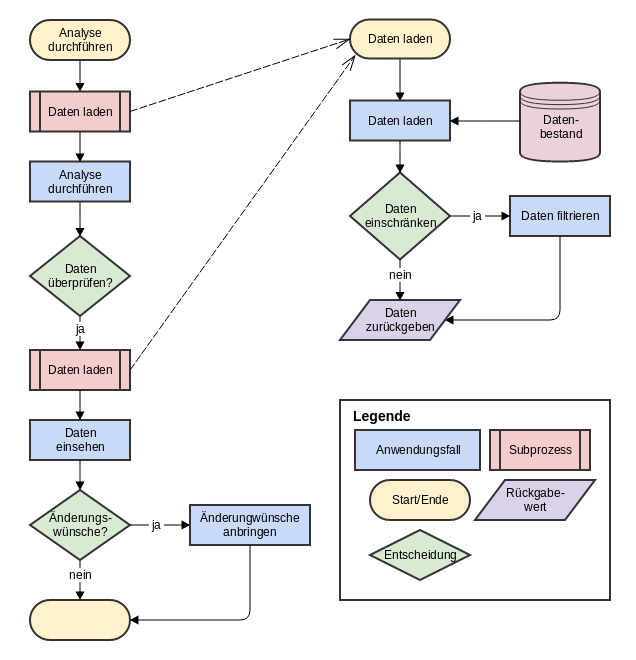
\includegraphics[width=0.8\textwidth]{images/flowchart}
	\caption{Ablauf}
	\label{fig:anfoderungsanalyse:ablauf:1}
\end{figure}

\subsection{Funktionale Anforderungen}
\label{sec:anforderungsanalyse:funktionaleanforderung}
Nachfolgend werden die funktionale Anforderungen an das Programm gestellt.

\begin{table}[H] 
	\caption{FA1: Häufigkeitsanalyse der Attribute}
	\centering
	\rowcolors{1}{tablebodycolor}{tablerowcolor}
	\label{fig:anforderungsanalyse:funktionaleanforderung:fa1}
	\begin{tabular}{ | l | L{10cm} | } 
		\hline 
		\rowcolor{tableheadcolor}
		\multicolumn{2}{|l|}{\bfseries ID: FA1} \\ \hline 
		Titel & Häufigkeitsanalyse der Attribute \\ \hline 
		Beschreibung & Das Programm muss für die Gewinnung neues Wissens aus der bisherigen Buchungen von Interhome gestaltet werden. Dazu sollen Algorithmen eingesetzt werden welche folgende beispielhaften Fragestellungen beantworten können:
		\begin{enumerate}
		\item Welche Attribute werden im Winter wenn schneit in der Schweiz gebucht?
		\item Welche Häuser im Tessin mit Sicht auf einen See werden am meisten gebucht?
		\end{enumerate}
		
		Als Antwort sollte der Algorithmus eine Liste von Attributen zurückliefern. Auf die obigen Beispiele könnte dies folgendes sein:
		\begin{enumerate}
		\item Objekte in Süditalien mit einem Pool.
		\item Luxushäuser mit einem Grill und 3 Zimmern.
		\end{enumerate} \\ \hline 
		Abhängigkeit & \\ \hline 
		Status & Offen \\ \hline 
	\end{tabular}
\end{table}

\begin{table}[H] 
	\caption{FA2: Nachvollziehbarkeit der Attributanalyse}
	\centering
	\rowcolors{1}{tablebodycolor}{tablerowcolor}
	\label{fig:anforderungsanalyse:funktionaleanforderung:fa2}
	\begin{tabular}{ | l | L{10cm} | } 
		\hline 
		\rowcolor{tableheadcolor}
		\multicolumn{2}{|l|}{\bfseries ID: FA2} \\ \hline 
		Titel & Nachvollziehbarkeit der Attributanalyse \\ \hline 
		Beschreibung & Die Resultate aus FA1 sollten nachvollziehbar sein. Es sollte dem Benutzer verständlich gemacht werden, wieso der Algorithmus diese Attribute gewählt hat. Jede Eigenschaft sollte demnach mit einer Anzahl oder einer Prozentzahl versehen sein. Zum Beispiel:
			\begin{enumerate}
			\item Sütitalien (223 von 319) und Pool (150 von 319)
			\item Luxushäuser (53\%), Grill (35\%) und 3 Zimmer (32\%)
			\end{enumerate} \\ \hline 
		Abhängigkeit & FA1 \\ \hline 
		Status & Offen \\ \hline 
	\end{tabular}
\end{table}

\begin{table}[H] 
	\caption{FA3: Häufigkeitsanalyse auf einer Untermenge der Daten}
	\centering
	\rowcolors{1}{tablebodycolor}{tablerowcolor}
	\label{fig:anforderungsanalyse:funktionaleanforderung:fa3}
	\begin{tabular}{ | l | L{10cm} | } 
		\hline 
		\rowcolor{tableheadcolor}
		\multicolumn{2}{|l|}{\bfseries ID: FA3} \\ \hline 
		Titel & Häufigkeitsanalyse auf einer Untermenge der Daten \\ \hline 
		Beschreibung & Eine Häufigkeitsanalyse solle gemäss FA1 auch auf einer Untermenge der Daten möglich sein. Der Benutzer soll befähigt werden den Datenbestand vor der Analyse einzuschränken. \\ \hline 
		Abhängigkeit & FA1 \\ \hline 
		Status & Offen \\ \hline 
	\end{tabular}
\end{table}

\begin{table}[H] 
	\caption{FA4: Stammdaten einsehen}
	\centering
	\rowcolors{1}{tablebodycolor}{tablerowcolor}
	\label{fig:anforderungsanalyse:funktionaleanforderung:fa4}
	\begin{tabular}{ | l | L{10cm} | } 
		\hline 
		\rowcolor{tableheadcolor}
		\multicolumn{2}{|l|}{\bfseries ID: FA4} \\ \hline 
		Titel & Stammdaten einsehen \\ \hline 
		Beschreibung & Um die Analyse der Daten zu validieren, sollte es möglich sein die Stammdaten einzusehen. Deshalb sollen im Programm alle Daten dargestellt werden können und vom Benutzer durchstöbert werden können. \\ \hline 
		Abhängigkeit & \\ \hline 
		Status & Offen \\ \hline 
	\end{tabular}
\end{table}

\begin{table}[H] 
	\caption{FA5: Untermenge der Stammdaten einsehen}
	\centering
	\rowcolors{1}{tablebodycolor}{tablerowcolor}
	\label{fig:anforderungsanalyse:funktionaleanforderung:fa5}
	\begin{tabular}{ | l | L{10cm} | } 
		\hline 
		\rowcolor{tableheadcolor}
		\multicolumn{2}{|l|}{\bfseries ID: FA5} \\ \hline 
		Titel & Untermenge der Stammdaten einsehen \\ \hline 
		Beschreibung & Eine Untermenge der Stammdaten soll gemäss FA3 eingesehen werden können. Diese sollen gleich wie in FA2 einschränkbar sein.  \\ \hline 
		Abhängigkeit & FA1 \& FA4 \\ \hline 
		Status & Offen \\ \hline 
	\end{tabular}
\end{table}

\begin{table}[H] 
	\caption{FA6: Mixed data types}
	\centering
	\rowcolors{1}{tablebodycolor}{tablerowcolor}
	\label{fig:anforderungsanalyse:funktionaleanforderung:fa6}
	\begin{tabular}{ | l | L{10cm} | } 
		\hline 
		\rowcolor{tableheadcolor}
		\multicolumn{2}{|l|}{\bfseries ID: FA6} \\ \hline 
		Titel & Mixed data types \\ \hline 
		Beschreibung & Da die Buchungen von Interhome numerische (z.B. Anzahl Personen, Geolocations) und kategorische Daten (z.B. Aircondition vorhanden?, Objekttyp) beinhalten, müssen die Algorithmen in der Lage sein mit beiden Datentypen umgehen zu können. \\ \hline 
		Abhängigkeit & \\ \hline 
		Status & Offen \\ \hline 
	\end{tabular}
\end{table}

\begin{table}[H] 
	\caption{FA7: Selbständigkeit}
	\centering
	\rowcolors{1}{tablebodycolor}{tablerowcolor}
	\label{fig:anforderungsanalyse:funktionaleanforderung:fa7}
	\begin{tabular}{ | l | L{10cm} | } 
		\hline 
		\rowcolor{tableheadcolor}
		\multicolumn{2}{|l|}{\bfseries ID: FA7} \\ \hline 
		Titel & Selbständigkeit \\ \hline 
		Beschreibung & Die Analyse der Attribute sollte selbständig Muster erkennen können. Es wird keine vorherige Eingabe vom Benutzer benötigt (ausser der Einschränkung der Daten). Siehe \gls{unsupervisedlearning} im Glossar. \\ \hline 
		Abhängigkeit & \\ \hline 
		Status & Offen \\ \hline 
	\end{tabular}
\end{table}

\begin{table}[H] 
	\caption{FA8: Algorithmen konfigurieren}
	\centering
	\rowcolors{1}{tablebodycolor}{tablerowcolor}
	\label{fig:anforderungsanalyse:funktionaleanforderung:fa8}
	\begin{tabular}{ | l | L{10cm} | } 
		\hline 
		\rowcolor{tableheadcolor}
		\multicolumn{2}{|l|}{\bfseries ID: FA8} \\ \hline 
		Titel & Algorithmen konfigurieren \\ \hline 
		Beschreibung & Der Benutzer soll die Möglichkeit besitzen, die Algorithmen zu konfigurieren. Deshalb sollen alle Parameter welche von den Algorithmen vorausgesetzt werden (siehe \cref{sec:recherche:algorithmen} \nameref{sec:recherche:algorithmen}) sowie das Gewicht zwischen numerischen und kategorischen Attributen der Distanzmessung (siehe \cref{sec:konzept:anwendungderalgorithmen:distanzmessung} \nameref{sec:konzept:anwendungderalgorithmen:distanzmessung}) angepasst werden können.
		Dies sind: 
		\begin{itemize}
			\item Apriori:
			\begin{itemize}
				\item Mindestsupport $minsup$
			\end{itemize}
			\item KPrototype:
			\begin{itemize}
				\item Anzahl Clusters $k$
			\end{itemize}
			\item DBScan:
			\begin{itemize}
				\item Radius $\epsilon$
				\item Minimum Anzahl an Instanzen $minpts$
			\end{itemize}
			\item Gewicht zwischen numerischen und kategorischen Attributen $\gamma$
		\end{itemize}
		 \\ \hline 
		Abhängigkeit & \\ \hline 
		Status & Offen \\ \hline 
	\end{tabular}
\end{table}


\subsection{Nicht funktionale Anforderungen}
\label{sec:anforderungsanalyse:nichtfunktionaleanforderung}
Nachfolgend sind die nicht funktionale Anforderungen an das Programm spezifiziert. Diese gehen nicht auf die Funktionalität der Applikation ein, sondern auf die Komplexität, Performanz, etc.

\begin{table}[H] 
	\caption{NFA1: Geschwindigkeit}
	\centering
	\rowcolors{1}{tablebodycolor}{tablerowcolor}
	\label{fig:anforderungsanalyse:nichtfunktionaleanforderung:nfa1}
	\begin{tabular}{ | l | L{10cm} | } 
		\hline 
		\rowcolor{tableheadcolor}
		\multicolumn{2}{|l|}{\bfseries ID: NFA1} \\ \hline 
		Titel & Geschwindigkeit \\ \hline 
		Beschreibung & Da das Programm explorativ verwendet werden soll, muss das Programm eine zügige Antwortszeit aufweisen. Deshalb soll die Attributanalyse innerhalb von 30 Sekunden Resultate liefern können. Die Algorithmen sollten daher maximal ein super-lineares Wachstum ($\mathcal{O}(n\,log\,n)$) aufweisen. \\ \hline 
		Abhängigkeit & \\ \hline 
		Status & Offen \\ \hline 
	\end{tabular}
\end{table}
\todo{apriori O(n log n)?}

\begin{table}[H] 
	\caption{NFA2: Komplexität}
	\centering
	\rowcolors{1}{tablebodycolor}{tablerowcolor}
	\label{fig:anforderungsanalyse:nichtfunktionaleanforderung:nfa2}
	\begin{tabular}{ | l | L{10cm} | } 
		\hline 
		\rowcolor{tableheadcolor}
		\multicolumn{2}{|l|}{\bfseries ID: NFA2} \\ \hline 
		Titel & Komplexität \\ \hline 
		Beschreibung & Verwendet wird das Programm von Interhome Mitarbeitern ohne Vorwissen im Data Mining. Deshalb sollte die Bedingung dementsprechend ausgelegt sein. \\ \hline 
		Abhängigkeit & \\ \hline 
		Status & Offen \\ \hline 
	\end{tabular}
\end{table}

\begin{table}[H] 
	\caption{NFA3: Modularität}
	\centering
	\rowcolors{1}{tablebodycolor}{tablerowcolor}
	\label{fig:anforderungsanalyse:nichtfunktionaleanforderung:nfa3}
	\begin{tabular}{ | l | L{10cm} | } 
		\hline 
		\rowcolor{tableheadcolor}
		\multicolumn{2}{|l|}{\bfseries ID: NFA3} \\ \hline 
		Titel & Modularität \\ \hline 
		Beschreibung & In Zukunft ist zu erwarten, dass das Programm um weitere Techniken des Data Mining erweitert werden soll. Deshalb sollte es Modular aufgebaut werden dass einfach weitere Algorithmen hinzugefügt werden. \\ \hline 
		Abhängigkeit & \\ \hline 
		Status & Offen \\ \hline 
	\end{tabular}
\end{table}

\begin{table}[H] 
	\caption{NFA4: Erweiterbarkeit der Daten}
	\centering
	\rowcolors{1}{tablebodycolor}{tablerowcolor}
	\label{fig:anforderungsanalyse:nichtfunktionaleanforderung:nfa4}
	\begin{tabular}{ | l | L{10cm} | } 
		\hline 
		\rowcolor{tableheadcolor}
		\multicolumn{2}{|l|}{\bfseries ID: NFA4} \\ \hline 
		Titel & Erweiterbarkeit der Daten \\ \hline 
		Beschreibung & Um die aktualität der Informationen zu gewährleisten, soll der Datenbestand in Zukunft leicht erweitert werden können. \\ \hline 
		Abhängigkeit & \\ \hline 
		Status & Offen \\ \hline 
	\end{tabular}
\end{table}
 
 \begin{table}[H] 
	\caption{NFA5: Kosten}
	\centering
	\rowcolors{1}{tablebodycolor}{tablerowcolor}
	\label{fig:anforderungsanalyse:nichtfunktionaleanforderung:nfa5}
	\begin{tabular}{ | l | L{10cm} | } 
		\hline 
		\rowcolor{tableheadcolor}
		\multicolumn{2}{|l|}{\bfseries ID: NFA5} \\ \hline 
		Titel & Kosten \\ \hline 
		Beschreibung & Falls ein bestehendes Programm eingesetzt wird, sollen folgende Kostenfaktoren beachtet werden: 
		\begin{itemize}
		\item Die Applikation sollte kostenlos einsetzbar sein. Sie benötigt demnach eine der folgenden Lizenzmodellen:
		\begin{itemize}
		\item OpenSource. Software kann verwendet und angepasst werden (siehe \url{https://opensource.org/licenses}).
		\item Freeware. Software kann verwendet, jedoch nicht angepasst werden.
		\item Studenten Lizenz. Software kann als Student kostenlos eingesetzt werden.
		\end{itemize}
		\item Die Entwicklung wird privat auf einem Linux Rechner durchgeführt, und Zeitweise auch bei der Arbeit auf Windows Computern welche von Hotelplan Management AG bereitgestellt werden.
		Demnach ist es nötig, dass die Software unter Linux sowie auch Windows gestartet werden kann.
		\item Da der Datenbestand 133'001 Einträge umfasst, muss die Plattform und das Lizenzmodel diese Anzahl an Items unterstützen.
		\end{itemize}\\ \hline 
		Abhängigkeit & \\ \hline 
		Status & Offen \\ \hline 
	\end{tabular}
\end{table}

